\section{February 7}
Last time, we left off after computing the integral for \( \mathbf{E} \), and we found that \( \Lambda \)
doesn't matter since it got canceled out after the computation. Now, we will discuss why this is true.      
Recall that the integral we wanted to compute was
\[
	\int_{z}^{\infty} e^{-i \omega r / c }\diff r
\]
First, let's define \( \theta = \frac{\omega}{r} \), so \( d\theta = \frac{\omega}{c}\diff r \), and our
integral becomes:
\[
	\int_{\theta_0}^{\infty}e^{-i \theta} \frac{c}{\omega} \diff \theta
\]
This integral lends itself to a very nice intuition: we can think of it as just adding up a bunch of complex
numbers together. Adding complex numbers in the complex plane can be thought of as vector addition, so
computing the integral is the same as adding up the vectors in the following diagram:

\begin{center}
	\begin{tikzpicture}
    \draw[thick,color=gray!70] (-1,-1.12) circle (1.5cm);
    \filldraw[white] (0,-1) -- (0,0) -- (1,0) -- (1,-1) -- cycle;
    \draw[color=orange!70!white] (0.2,0) arc (0:-52.12:0.2cm) node[midway,right,yshift=-0.05cm,scale=0.5] {$\theta_0$};
    \draw[thick,stealth-stealth] (0,-3) -- (0,3);
    \draw[thick,stealth-stealth] (-4,0) -- (4,0);
    \draw[thick, color=orange!70!white,-stealth] (0,0) -- (0.35,-0.45) node[right,yshift=0.1cm,scale=0.5] {$e^{-i\theta_0\left(\frac{c}{\omega}d\theta\right)}$};
    \draw[densely dotted] (0.35,-0.45) -- (0.6,-0.77);
    \draw (0.475,-0.61) arc (-52.12:-74.74:0.2cm) node[right,scale=0.35,yshift=-0.1cm] {$d\theta$};
    \draw[thick,color=blue!60!cyan!80,-stealth] (0.35,-0.45) -- (0.5,-1) node[right,scale=0.5] {$e^{-i(\theta_0+d\theta)\left(\frac{c}{\omega}d\theta\right)}$};
\end{tikzpicture}
\end{center}

Essentially, we start with a vector at an angle \( \theta_0 \), then we continually add vectors of the same
"length" together, all the while changing the angle slightly by \( d\theta \). If we continue this process,
we eventually loop back around to the origin. What this ultimately means is that when we integrate from \(
\theta_0 \) to infinity, we end up traversing this loop infinitely many times, which is why the integral
diverges. 

Now, when we add a \( \Lambda \) term, what happens is that the "length" of the vector we add each time
decreases, so instead of the addition coming out to a circle, it ends up as a \textit{spiral}. Further, if \(
\eta(\theta)\) decreases slowly enough (so make \( \Lambda \) sufficiently large, but not infinite), then the
integral will converge at the \textit{center} of the earlier circle. So, the integral looks something like
the following diagram:

\begin{center}
	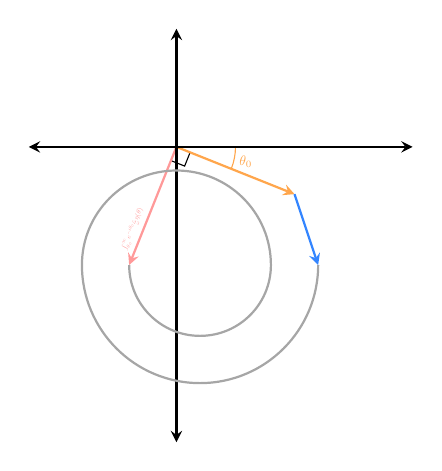
\begin{tikzpicture}[scale=1.5]
    \draw[rotate=-21.8] (0.125,0) -- (0.125,-0.125) -- (0,-0.125);
    \draw[thick,red!40!white,-stealth] (0,0) -- (-0.4,-1) node[midway,left,scale=0.25,rotate=68,yshift=0.5cm,xshift=-0.2cm] {$\int_{\theta_0}^{\infty}e^{-i\theta_0}\frac{c}{\omega}\eta(\theta)$};
    \draw[thick,orange!70!white,-stealth] (0,0) -- (1,-0.4);
    \draw[color=orange!70!white] (0.5,0) arc (0:-21.8:0.5cm) node[midway,right,yshift=-0.05cm,scale=0.5] {$\theta_0$};
    \draw[thick,color=blue!60!cyan!80,-stealth] (1,-0.4) -- (1.2,-1);
    \draw[thick,stealth-stealth] (0,-2.5) -- (0,1);
    \draw[thick,stealth-stealth] (-1.25,0) -- (2,0);
    \draw[thick, color=gray!70] (-0.4,-1) arc (-180:0:0.6cm) arc (0:180:0.8cm) arc (-180:0:1cm);
\end{tikzpicture}
\end{center}


What does the integral converge to? From the geometry, the resulting vector is perpendicular to the initial
vector, so we have:
\[
	\int_{\theta_0}^{\infty} e^{-i \theta} \frac{c}{\omega}\eta(\theta) = Re^{-i (\theta_0 + \pi / 2)}
\]
To find the radius \( R \), we also use geometry, to get \( R \diff \theta = \frac{c}{\omega} \diff \theta
\), so we get \( R = \frac{c}{\omega} \). This now explains why \( \Lambda \) doesn't matter, since whatever
value of \( \Lambda \) chosen, we will converge to the center of the circle. So, the integral becomes:
\[
	\int_{z}^{\infty}e^{-i \omega r / c} \diff r = \int_{\theta_0}^{\infty}e^{-i \theta}\frac{c}{\omega}
	\diff \theta = R e^{-i \left( \theta_0 + \frac{\pi}{2} \right)} = \frac{c}{\omega}(-i) e^{-i \omega z / c}
\]
So now applying this to the integral for \( \mathbf{E} \), we get the result from last lecture:
\[
	\mathbf{E} = \frac{q \omega x_0 \eta_0}{2 \epsilon_0 c^2} \Re\left[ \frac{c}{i} e^{i \omega \left( t -
	\frac{z}{c} \right)} \right]
\]
\subsection{The "Delayed" Wave}
Now, let's consider the following system, with a source which emits an electric field \(
\mathbf{E}_\text{source} \) and a point \( P \) far away, and we place a thin sheet of linear media in
between the two. The sheet has thickness \( \Delta z \). Phenomenologically, we know that light travels
slower in glass compared to vacuum, by a ratio of \( v = \frac{c}{n} \), so the wave will take extra time to
arrive at \( P \). In particular, the extra time is given by:
\[
	\Delta t = \frac{\Delta z}{v} - \frac{\Delta z}{c} = (n - 1) \frac{\Delta z}{c}
\]
So, with the glass in between, we have to add this \( \Delta t \) term into the exponential, and
thus:\footnote{We are being a bit lazy with the notation here, \( \mathbf{E} \) should be a vector quantity
but we only care about its magnitude for now so we'll treat it as a scalar.}
\[
	E(t, z) = E_0 e^{i \omega\left( t - \Delta t - \frac{z}{c} \right)} = E_0 e^{i \omega \left( t - \frac{n
	- 1}{c} \Delta z - \frac{z}{c} \right)}
\]
If the slab is assumed to be very thin, then we can extract the \( \Delta z \) term, and Taylor expand it:
\begin{align*}
	E(t, z) &= E_0 e^{-i \omega \frac{n - 1}{c} \Delta z} e^{-i \omega \left( t - \frac{z}{c} \right)}\\
	&= E_0 \left( 1 - i \frac{n - 1}{c}\Delta z \right) e^{i \omega\left(t - \frac{z}{c}\right)} \\ 
	&= E_0 e^{i \omega \left( t - \frac{z}{c} \right)} - \frac{i (n -1) \omega \Delta z}{c}E_0 e^{i
	\omega\left( t - \frac{z}{c} \right)}
\end{align*}
The first term can be thought of as just \( \mathbf{E}_\text{source} \), while the second term can be thought
of as the wave produced by the charges in the material.  

\subsection{A Microscopic Model}
Now, let's consider what happens in the glass itself. When a sinusoidal source electric field \(
\mathbf{E}_\text{source} = E_0 e^{i \omega t}\) contacts the glass, it will oscillate the charges inside the glass.
Microscopically, each dipole in the glass is in a potential well, which usually looks like the following:

\begin{center}
	\begin{tikzpicture}[line cap=round]
		% Axis
		\draw[thick, -latex] (-2ex,0) -- (8,0) node[below] {\( x \)};
		\draw[thick, -latex] (0,-2.5) -- (0,5) node[left] {\( U \)};	
		
		% Plot Function
		\draw[domain=0.177:7.5, samples=400, variable=\r, very thick, red] plot ({\r},{0.3/(\r*\r)-0.9/\r});
		
		% Dashed
		\draw[dashed] (2/3,0) -- +(0,-0.65) node[pos=0, above] {\( x_\text{eq} \)};
	\end{tikzpicture}
\end{center}

Here \( x_\text{eq} \) marks an equilibrium point, around which the charge oscillates. It is a (global)
minimum, so the first derivative is zero, and hence its Taylor expansion around \( x_\text{eq} \)is:
\[
	U = U(x_\text{eq}) + \frac{1}{2} U''(x_\text{eq}) (x - x_\text{eq})^2
\]
This should be somewhat familiar from classical mechanics. The equation of motion, according to 
Newton's equation, is given by:
\[
	m \ddot x = - m \omega_0^2 x + q E_0 e^{i \omega t}
\]
Intuitively, when the electric field gives the charge some energy, the charge will oscillate with a
sinusoidal motion as well, so let \( x(t) = x_0 e^{i \omega t} \). Putting this ansatz into the equation of
motion, we get:
\[
	-m \omega^2 x_0 e^{ i \omega t} = - m \omega_0^2 x_0 e^{i \omega t} + q E_0 e^{ i \omega t} \implies x_0
	= \frac{qE_0}{m(\omega_0^2 - \omega^2)}
\]
This implies that the motion for \( x(t) \) is:
\[
	x(t) = \frac{qE }{m(\omega_0^2- \omega^2)}e^{ i \omega t}
\]
Combining this result with what we have at the end of last lecture for
\( \mathbf{E} \), we have the following equation for the electric field of the dipole:
\[
	E_\text{dipole} = \Re\left[ -i \frac{q \omega}{2 \epsilon_0 c} \frac{q E_0 N \Delta z}{m(\omega_0^2 -
	\omega^2)}e^{i \omega\left( t - \frac{z}{c} \right)} \right]
\]
Here, \( N \Delta z = \eta_0 \), which is the density of charges per volume.  

